\documentclass[11pt,a4paper]{scrartcl}
\usepackage{color}
\usepackage{ifthen}
\usepackage{ifpdf}
\usepackage[headings]{fullpage}
\usepackage{listings}
\lstset{language=Java,breaklines=true}
\ifpdf \usepackage[pdftex, pdfpagemode={UseOutlines},bookmarks,colorlinks,linkcolor={blue},plainpages=false,pdfpagelabels,citecolor={red},breaklinks=true]{hyperref}
  \usepackage[pdftex]{graphicx}
  \pdfcompresslevel=9
  \DeclareGraphicsRule{*}{mps}{*}{}
\else
  \usepackage[dvips]{graphicx}
\fi

\newcommand{\entityintro}[3]{%
  \hbox to \hsize{%
    \vbox{%
      \hbox to .2in{}%
    }%
    {\bf  #1}%
    \dotfill\pageref{#2}%
  }
  \makebox[\hsize]{%
    \parbox{.4in}{}%
    \parbox[l]{5in}{%
      \vspace{1mm}%
      #3%
      \vspace{1mm}%
    }%
  }%
}
\newcommand{\refdefined}[1]{
\expandafter\ifx\csname r@#1\endcsname\relax
\relax\else
{$($in \ref{#1}, page \pageref{#1}$)$}\fi}
\date{\today}
\chardef\textbackslash=`\\
\usepackage{pdfpages}
\usepackage[utf8]{inputenc}
\usepackage[T1]{fontenc}
\usepackage[german]{babel}
\usepackage{hyperref}
\hypersetup{
	pdftitle={Pflichtenheft},
	bookmarks=true,
}
\usepackage{csquotes}

\usepackage{fancyhdr}%<-------------to control headers and footers
\usepackage[a4paper,margin=1in,footskip=.25in]{geometry}
\fancyhf{}
\fancyfoot[C]{\thepage} %<----to get page number below text
\pagestyle{fancy} %<-------the page style itself

\usepackage{xcolor}
\usepackage{framed}
\definecolor{shadecolor}{RGB}{220,220,220}
\usepackage{float}


\title{Android GO! App - Implementierung}
\author{Gruppe 3}
\date{20.08.17}

% define custom lists
\usepackage{enumitem}
\usepackage{lipsum}

\begin{document}

\begin{titlepage}
	\begin{center}
	{\scshape\LARGE \bfseries Implementierungsbericht \par}
	\vspace{1cm}
	{\scshape\Large Praktikum der Softwareentwicklung \\ Sommersemester 2017\par}
	\vspace{1.5cm}
	{\huge\bfseries Android GO! App\par}
	\vspace{2cm}
	{\Large\itshape - Gruppe 3 -\par}
	\vfill
	{\bfseries erstellt von:\par}
	Arsenii Dunaev \\
	Florian Kröger \\
	Tina Maria Strößner \\
	Volodymyr Shpylka \\	
	\vfill
	% Bottom of the page
	{\large 20.08.17 \par}	
	\end{center}
\end{titlepage}

\newpage

\tableofcontents

\newpage

\section{Änderungen zum Pflichtenheft und Entwurf}
\begin{enumerate}
	\item \textbf{Hinzufügen von Service-Klassen in der Service-Layer des Servers}\\
	Der Business-Layer des Servers wurden die Klassen \textit{userService, GroupService} und \textit{GoService} hinzugefügt. Diese dienen hauptsächlich der klareren Strukturierung zwischen den Aufgaben der restController und der Dao-Klassen. Anstatt direkt auf die Persistence-Layer zuzugreifen, interagieren die RestController-Klassen nur noch mit dem für sie zuständigen Service. In den Service-Klassen wird das Anpassen von Daten für die Umwandlung zu JSON oder zur Persistierung übernommen, sowie die Benachrichtigung der Observer, die vorher in den DAO-Klassen stattgefunden hat.
	
Durch das Hinzufügen dieser Klassen haben sowohl die RestController als auch die DAO-Klassen nur noch einen Verantwortlichkeitsbereich, um den sie sich kümmern müssen. Jeglicher Code der nur zur Umwandlung und Verwaltung der Daten dient, kann an die Service-Klassen ausgelagert werden.

	\item \textbf{Zusätzliche Client-Entity Klassen}\\
	Da sich die Anforderungen an die Datenmodellierung auf dem Server und auf dem Client stark unterscheiden, wurden jeweils unterschiedliche Entity-Klassen zur Modellierung der Entitäten verwendet. Um die Anwendungen trotzdem miteinander kompatibel zu machen, verfügt der Server zusätzlich über ClientEntity-Klassen, die die Datenmodellierung auf den Clients entsprechen.
	
	Die Verwendung dieser Klassen erlaubt das einfache Parsen von JSON-Objekten, die über die Client-Server Schnittstellen übertragen wurden. Die Umwandlung von ClientEntities zu ServerEntities übernehmen die entsprechenden Service-Klassen. Im Quellcode lassen sich Instanzen der ClientEntity-Klassen an dem Buchstaben c im Variablennamen erkennen (z.B. \textit{cGroup}).
	
	\item \textbf{Zusätzliche Klasse \textit{Utility} fürs Clustering}\\
	Da zum Clustering nicht eine Bibliothek verwendet müssen einige Funktionen erfüllt werden, die den Code um einiges unübersichtlicher machen würden. Deswegen gibt es die Utility-Klasse, die einige Methoden zusammenfassen, die vom Clusteringalgorithmus \textit{DBScan} aufgerufen werden.
	
	\item \textbf{Min Android Version} \\
	
	Die minimale Android Version ist jetzt API 24, weil da viele Shortcuts und nützliche Sachen von Google zur Verfügung gestellt werden, die helfen viele Sonderfälle zu vermeiden.	
	
	\item \textbf{F0010}\\Standort Erlaubnis wird nicht zur Registrierungszeit abgefragt, sondern zur Laufzeit, gleich wenn man die Standortverfolgung braucht. Macht nichts aus, da User die Standortverfolgung außerhalb der App auch ausschalten kann.
Wenn der Benutzer die Berechtigung nicht gibt, dann zeigt die App einen Dialog, dass erklärt, dass man die Berechtigung in Geräteeinstellungen geben muss, damit die App wieder funktioniert. Bis man die Berechtigung gibt ist die ganze Funktionalität nicht zugänglich.
\item \textbf{F0020}\\
F0020 Bemerkung: beim Einloggen braucht man kein E-Mail und Passwort einzugeben, wenn man schon in sein Google-Account eingeloggt ist. Man wählt nur den Google Account, mit dem man sich anmelden möchte.
\item \textbf{F0070}\\
F0070 Gruppenbeschreibung war ein Wunschkriterium, wurde aber implementiert.
Wenn man den Gruppeneintrag aus der Liste aller Gruppen anklickt, wird dem Benutzer die Gruppenansicht angezeigt. Da sieht man nur die Gruppenname und Liste aller GOs. Um die Mitglieder und Beschreibung zu sehen muss man die Gruppenname oben anklicken, dann wird dem Benutzer die Gruppendetails Ansicht angezeigt.

\item \textbf{F0080}\\ "Gruppe erstellen" ist mit dem runden Button unten rechts dargestellt.

\item \textbf{F0090}\\ "Gruppe verlassen" Button befindet sich in der Gruppendetails Ansicht. Wenn Admin die Gruppe verlässt, dann wird die Gruppe gelöscht, da wir jetzt keinen Wunschkriterium implementiert haben, wo man einen neuen Admin zuweist.

\item \textbf{F0110}\\ Wie gesagt, Gruppenbeschreibung ist jetzt implementiert.

 \item \textbf{F0120}\\ Die Anfragen werden jetzt den Administratoren nicht angezeigt.

\item \textbf{F0130}\\ Wenn der Administrator den Mitglied-Eintrag in der List anklickt und hält, dann erscheint ein Context Menu, um diesen Benutzer zu entfernen.

\item \textbf{F0170}\\ Informationen werden immer angezeigt, da der User sowieso den Zustand frei wechseln darf, also wäre nur unnötiger Aufwand.

\item \textbf{F0180}\\ Beschreibung wurde implementiert. Zielpunkt ist nicht mehr optional.

\item \textbf{F0200}\\ Jeder Status darf die Cluster sehen.

\item \textbf{F0210}\\ + GO Beschreibung

\item \textbf{Client Repository Singletones}\\
	Alle Repository Klassen auf dem Client sind als Singletones implemetiert, weil man nur eine einzige Instanz braucht, die für jeden Level (Main Level,  Group Level, Go Level, User Level) die Kommunikation mit dem Server behandelt. Also mehrere Instanziierungen sind zu vermeiden, damit die Anfragen nur einmal Worst Case ausgeführt werden.
	
\item \textbf{Client ViewModel Singletones}\\
Die ViewModel Klassen sind auch als Singletones implementiert, weil es in der entwurfsphase nicht offensichtlich war, dass die ViewModels die Activity-Lifecycle überleben. Also auch wenn die Activities zerstört und neu erzeugt werden, bleibt dasselbe ViewModel für den Activity Typ zuständig. Die Activities nehmen dann die Daten von den ViewModels. Dazu brauchen wir auch nicht viele Instanzen von eimen ViewModel. Und die werden von Android auch so gedacht, als singletones benutzt zu werden.

\item \textbf{Änderungen zu Activity Klassen}\\

Hauptsächlich sind die Activity Klassen geblieben, die im Entwurf waren, und dazu haben wir auch Activities, Fragments, Dialogs hinzugefügt, die den User-Experience vervollständigen, aber nicht die Hauptziel von dem Entwurf sind, wie z.B. (Bearbeiten das, was in der jetzigen Activity steht, erzeuge eine Entity).

Solche Activities wie EditGroupActivity, CreateGroupActivity, AddMember, also "lightweight" Activities, die nicht viel Logik haben, sind einfach als Dialogs implementiert, da diese leichter zu managen sind in Scope von einer anderen "heavyweight" Activity, wie z.B. GroupDetailActivity. \\

Einige Sachen wurden zu Fragmenten, wie z.B. GoMapFragment und GoDetailsFragment, die man in der GoDetailActivity benutzt, weil man da swipen zwischen zwei Fragmenten unterstützen muss.

\item \textbf{Datenhierarchie auf dem Client}\\

Daten sind folgendermaßen auf dem Client gestaltet: der Main Speicher von allen Daten während der Session auf dem User-Smartphone ist die GroupRepository Klasse. Da befinden sich alle Daten in einer custom LiveData Klasse. Diese Daten beobachtet die Klasse GroupListViewModel - das ist die ViewModel der "main" GroupListActivity Klasse, die ein Entry-Point zu der Go-App ist. \\

Nach dem Starten werden die Daten von der GroupListViewModel aus der GroupRepository gefetcht, danach updated die Repo ihre Daten, und da die ViewModel diese beobachtet, bekommt sie immer aktuelle Daten nachher. Alle Anfragen in der App werden durch Repositories zu dem Server gerouted, und dann die Daten die in Responses ankommen, werden immer bei der GroupRepository updated, und dann hat die ganze App durch die Beobachters den aktuellen Stand.\\

GroupViewModel, GoViewModel bekommen ihre Daten, von der GroupListViewModel, also "main" ViewModel und nicht von den Repositories. Somit sind diese ViewModels auch von GroupRepository abhängig und daher konsistent. Die entsprechende Repositories zu Group und Go dienen nur dazu, um die Anfragen an den Server zu routen. Die Daten werden aber dann in GroupRepository updated.\\

Wenn man einen asynchronen Aufruf macht, wird es über die entsprechende Repository geschickt, und dann über Commands empfangen, und die Commands wählen passende Methoden, um die neuen Daten auf dem Client zu speichern.\\

Zu jedem Command gibt es meistens einen Methode in der GroupRepository, wie z.B. GoAddedCommand -> GroupRepository.onGoAdded(Go go, groupId). In allen on...() Methoden werden die Daten von Command Klassen in GroupRepository gesetzt und danach weiter durch die App propagiert.

\item \textbf{LiveData Klassen}\\

Zu allen LiveData<> Klassen wurden Unterklassen erstellt, damit die postValue und setValue Methoden sichtbar sind, weil genau diese Methoden triggern die Beobachter dann.

\item \textbf{Methoden bei Repository}\\

Es gibt 3 Methoden bei der Repository Klasse. Wir dachten, dass die ziemlich sinnvoll da waren, aber als wir die Implementierung angefangen haben, waren die Methoden ein bottleneck für uns, und wir habe es als sinnvoll gehalten, die Daten anders zu routen. Am Ende sind wir dazu gekommen, dass diese 3 Methoden unnützlich sind, da wir bis zum Ende diese nicht benutzt haben und es kein Grund sich ergab, diese irgendwann zu benutzten.
	
\end{enumerate}

\newpage

\section{Wunsch und Musskriterien}

\newpage

\section{Ablauf}

Zu Beginn der Implementierungsphase wurde das Projekt in 2 Teile aufgeteilt:

\textit{Server} und \textit{Client}

Es wurde jeweils ein Vorgehensplan aufgestellt für die kommenden Wochen.

\subsection{Server}

\begin{enumerate}
	\item \textbf{Zu Beginn:} Datenbank
	
	\item \textbf{Mittig:} DAOs
	
	\item \textbf{Schlussendlich:} Clustering, Observer, RestController
	
\end{enumerate}

\subsection{Client}
\begin{enumerate}
	\item \textbf{Zu Beginn:} Activities 

	\item \textbf{Mittig:} Daten für Activities

	\item \textbf{Schlussendlich:} Vorbereitung zur Verbindung mit dem Server
\end{enumerate}

Zum Ende hin sollte dann die Zusammenarbeit von Server und Client getestet werden.

\subsection{Verzögerungen}
Zu Beginn verlief Alles Planmäßig, allerdings kam es später vermehrt zu Verzögerung an mehreren Enden.
Aufgrund von Misskommunikation mussten viele Klassen verbessert oder neu geschrieben werden um den Server und Client miteinander arbeiten zu lassen.
 
Als Folge hat sich das Testen beider als Ganzes sehr verzögert und nicht für ein gründliches und vollständiges Testen sämtlicher Klassen und Methoden ermöglicht, was wiederum zu weiteren Verzögerungen geführt hat.

\newpage

\section{Unittests}

\subsection{Server}

\subsubsection{Testdaten}\label{Testdaten}
Für die Unittests des Servers wurden Testdaten verwendet, die sowohl in eine Testdatenbank gespeichert wurden, als auch als Java-Objekte über die Klasse 'TestData'.

\subsubsection{Tests für Observer-Klassen}
Die Tests der Observer-Klassen sind in der Testklasse 'ObserverTest' zusammengefasst. Für jede Observer-Klasse muss die öffentliche Methode \textit{update()} getestet werden.
Um die Korrektheit der Methode zu überprüfen, wird getestet, ob der Methodenaufruf \textit{send(String data, EventArg arg, Set<UserEntity> receiver)} korrekt ausgeführt wird. Korrekt hei"st in diesem Fall, dass der Methodenaufruf erfolgt und die übergebenen Argumente den Vorgaben entsprechen.

Das Argument \textit{data} ist ein JSON-String, der wie im Entwurfsdokunment beschrieben aufgebaut ist. Das Argument \textit{arg} ist ein Element des Enums \textit{EventArg} und repräsentiert, die aufgetretene Änderung. Das Set \textit{receiver} enthält alle User, an die eine Benachrichtigung geschickt werden soll.

Für die Tests der Klasse 'ObserverTest' werden Mock-Objekte der Dao-Klassen verwendet. Diese sind mit dem Framework 'Mockito' erstellt und so konfiguriert, das bei Aufruf der Methode \textit{get({Long | String} key)} (Methode des AbstractDao Interfaces) ein zuvor definiertes TestObjekt zurückgegeben wird. Die verwendeten Testobjekte stammen aus der Klasse 'TestData', die für die Bereitstellung von Testobjekten zuständig ist (siehe \ref{Testdaten}).

Das FcmClient-Attribut der Observer-Klassen wird in den Test ebenfalls gemockt und so konfiguriert, das bei einem Methodenaufruf von \textit{send(...)} die übergebenen Argumente in Feldern der ObserverTest-Klasse gespeichert werden, so dass diese anschließend mit den erwarteten Werten verglichen werden können.

Die Ergebnisse, die bei Testausführung erwartet werden, sind als statische Felder in der Testklasse gespeichert. Dazu gehören die erwarteten JSON-Strings und die Receiver der send()-Methode.
Die erwarteten Ergebnis wurden, teils händisch, anhand des Entwurfsdokuments aus den in TestData definierten Testdaten generiert. Sie sind nur gültig, solange keine Änderungen an diesen Daten vorgenommen werden.

\subsubsection{Tests für RestController-Klassen}
Die Tests der Klassen User-, Group- und GoRestController sind jeweils darauf zu überprüfen, ob die Calls an die Rest-Ressourcen richtig interpretiert und ausgeführt werden. Dazu gehört das korrekte Auslesen von Methodenparametern aus der URI der Rest-Ressource und JSON Strings aus dem Request-Body.

Die Rest API wird bei dem Tests mithilfe des Spring Boot Starter Test-Frameworks simuliert. Dadurch kann sowohl das Mapping von Rest-Ressourcen, als auch die Methodenaufrufe in den Controller-Klassen getestet werden.

Um die Korrektheit der Methodenaufrufe zu überprüfen, wird in jeder Testmethode der Methodenaufruf an die jeweilige Service-Klasse überprüft, die übergebenen Parameter, sowie die HTTP-Response, die zurückgegeben wird. Die dabei verwendeten Testdaten, die aus der TestData-Klasse stammen, wurden mithilfe eines Rest-Clients auf Korrektheit überprüft.

\subsubsection{Tests für Service-Klassen}
Für die Klassen User-, Go- und GroupService wurde je eine Testklasse erstellt, in denen sämtliche Methoden getestet werden. Da die meisten dieser Methoden \textit{void}-Methoden sind, kommt es vor allem darauf an, zu testen, ob der richtige Methodenaufruf auf dem jeweiligen Dao-Objekt erfolgt und ob jeweils er passende Observer benachrichtigt wird.

Für die Realisierung dieser Tests wurden das Testframework Mockito, sowie Daten der \textit{TestData}-Klasse verwendet.

\subsubsection{Tests für Entity-Klassen}
Die Entity-Klassen bestehen hauptsächlich aus Getter- und Setter-Methoden, die aufgrund ihrer Einfachheit nicht extra getestet werden. Die einzigen Methoden, die aus den Entity-Klassen getestet werden, sind jeweils die Methoden \textit{equals()} und \textit{hashCode()}. Ob der \textit{equals()}/\textit{hashCode()} Contract eingehalten wird, wird mittels des EqualsVerifier getestet.

\subsection{Test für Klassen bezogen aufs Clustering}
Im Falle vom Clustering müssen die Klassen \textit{Utility}, \textit{DBScan}, \textit{GoClusterStrategy} und \textit{LocationService}. Da die Klassen sehr rechenlastig sind werden sie darauf getestet ob ein richtiges Resultat rausgegeben wird.

Da die Klassen eng miteinander verwoben sind muss Mockito eingesetzt werden um die Klassen halbwegs isoliert testen zu können.

\newpage

\section{Testabdeckung}
\subsection{Server}


\begin{center}
	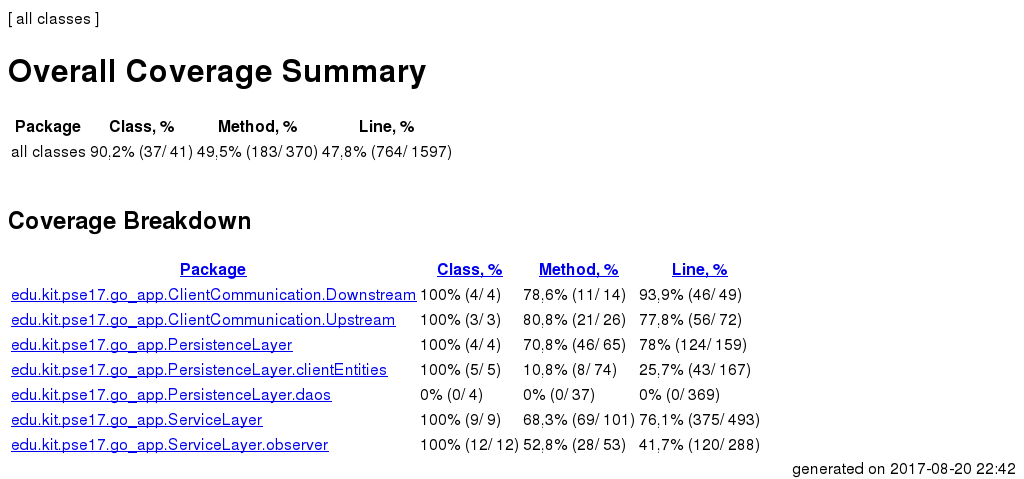
\includegraphics[width=1.0\linewidth]{ServerTestCoverage}
\end{center}



\end{document}
\grid
